\documentclass[a4paper,11pt,fleqn]{article}%fleqn pour aligner les equations à gauche
\usepackage{../../Styles/Exercice}


\newcommand{\chnum}{Chapitre 16}
\newcommand{\chtitle}{Énergie lumineuse et effet photoélectrique}
\newcommand{\dtype}{Exercices}

\begin{document}
	\maketitle
Données pour tous les exercices :
\begin{itemize**}
    \item \textbf{Constante de Plank : } $h=\SI{6.63E-34}{\joule\second}$
    \item \textbf{Unité d'énergie :} $\SI{1}{eV} = \SI{1.60E-19}{\joule}$
    \item \textbf{Célérité de la lumière dans le vide :} $c=\SI{3.00E8}{\meter\per\second}$
\end{itemize**}

\begin{multicols}{2}
\section{Émission d'un photon}
Un atome de sodium se désexite en émettant un photon d'énergie $E=\SI{2.11}{eV}$.\\
Calculer la longueur d'onde du rayonnement émis.

\section{effet photoélectrique}
on produit un effet photoélectrique sur un morceau d'étain de fréquence seuil $\nu_0 = \SI{1,1E15}{\hertz}$.\\
Indiquer ce que l'on observe pour un rayonnement de fréquence $\nu<\nu_0$ et pour un rayonnement de fréquence $\nu>\nu_0$.

\section{Photosynthèse}
Les plantes créent de la matière organique à partir du dioxyde de carbone \ce{CO2(g)} présent dans l'air et de l'énergie lumineuse, ce qui peur permet de pousser.
\begin{center}
     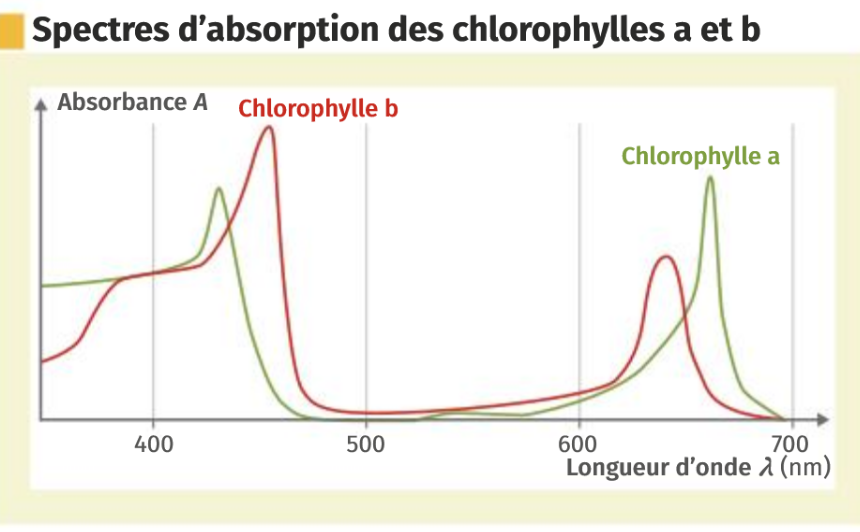
\includegraphics[width=.45\textwidth]{Ressources/TSPE_C16_fig2.png}
\end{center}
\begin{enumerate}
    \item A partir du document ci-dessous, déterminer les longueurs d'onde pour lesquelles les photons sont principalement absorbés par les feuilles.
    \item Calculer les énergies des photons utilisés par les plantes vertes au cours de la photosynthèse.\\
\end{enumerate}

\section{Nombre de photons venant du Soleil}
Par beau temps, le flux surfacique (ou irradiance) vaut environ \SI{0.50}{\kilo\watt\per\meter\squared}.
\begin{enumerate}
    \item Calculer l'énergie moyenne d'un photon solaire.
    \item Calculer l'ordre de grandeur du nombre de photons reçus par un capteur de surface \SI{1}{\meter\squared} pendant \SI{1}{s}.
\end{enumerate}

\section{Effet photoélectrique sur le titane}
Pour le titane, me travail d'extraction est $\Phi = \SI{4.1}{eV}$.
\begin{enumerate}
    \item Calculer la longueur d'onde seuil du titane.
    \item Expliquer ce qui se passe lorsque l'on éclaire une lame de titane par un rayonnement de longueur d'onde \SI{450}{nm}. Même question pour \SI{250}{nm}.
\end{enumerate}

\section{Rendement quantique}
On éclaire la cathode d'une cellule photoélectrique au potassium par une source lumineuse de longueur d'onde $\lambda=\SI{490}{nm}$ et dont la puissance du rayonnement vaut $P=\SI{4.5E-7}{W}$. le travail d'extraction du potassium est $\Phi=\SI{2.29}{eV}$.
\begin{enumerate}
    \item Calculer l'énergie des photons et vérifier que l'extraction des électrons est possible.
    \item Calculer le nombre de photons reçus en \SI{1}{s}.
    \item Sachant que l'on obtient une intensité $I= \SI{2,00E-8}{A}$ lorsque tous les électrons arrachés à la cathode arrivent à l'anode, calculer le nombre d'électrons extraits de la cathode en \SI{1}{s}.
    \item Déterminer le rendement quantique de la cellule, c'est-à-dire le rapport du nombre d'électrons extraits sur le nombre de photons reçus par la cathode.
\end{enumerate}
\end{multicols}


\section{Charge d'une batterie}
On souhaite mettre en place une installation photovoltaïque sur le toit d'une maison à Avignon. La consommation d'électricité étant bien plus faible en journée qu'en soirée, il est nécessaire d'installer une batterie.\\
Dans le~\ref{fig1}, on donne les caractéristiques courant-tension des panneaux utilisés pour différentes irradiances (ou flux lumineux surfaciques). On réalise l'étude pour une journée du mois de juillet.
\begin{enumerate}
    \item Si l'on considère que, toute la journée, l'irradiance reste constante et égale ) \SI{1,0}{\kilo\watt\per\meter\squared}., déterminer la durée moyenne d'ensoleillement quotidien.
    \item \ref{fig1} Sachant que le tension aux bornes de la batterie est de \SI{24}{V}, déterminer la valeur du courant fourni par le panneau à la batterie.
    \item En déduire la charge électrique $Q_p$ fournie par le panneau solaire à) la batterie en une journée. Donner le résultat en ampère-heure (\unit{\ampere\hour}).
    \item la batterie utilisée a une capacité électrique $Q_{max}=\SI{230}{\ampere\hour}$ et un rendement en charge $\eta=\SI{85}{\percent}$. Déterminer le nombre de panneaux solaire nécessaires pour charger entièrement la batterie en une journée durant le mois de juillet à Avignon.
\end{enumerate}
Donnée : \textbf{Energie de rayonnement surfacique reçue durant une journée du mois de juillet à Avignon :} $\epsilon = \SI{6,6}{\kilo\watt\hour\per\meter\squared}$

\begin{figure}[h!]
    \subfloat[Caractéristiques intensité-tension]{
    \centering
    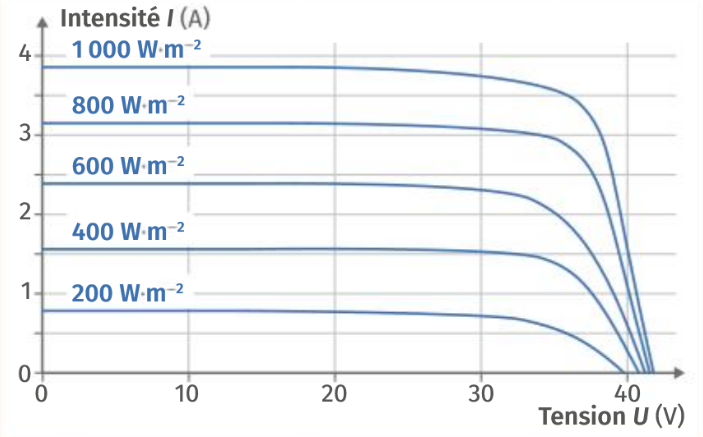
\includegraphics[width=.49\linewidth]{Ressources/TSPE_C16_fig3.png}
    \label{fig1}
    }
    \subfloat[Capacité électrique]{\raisebox{12ex}{\begin{minipage}{.49\linewidth}
    La capacité électrique d'une batterie est la charge maximale qu'elle peut fournir. Le rendement en charge définit le rapport entre la charge électrique restituée lors de la décharge et la charge électrique reçue lors de la charge.
    \end{minipage}}
    \label{fig2}}
    
\end{figure}
\end{document}